\hypertarget{haskell}{%
\section{Haskell - Interactive Programming}\label{haskell}}

\hypertarget{io-functions}{%
\subsection{IO functions}\label{io-functions}}

It is possible to interact with the real world from Haskell. You are
able to develop functions which return an IO of a type.

\begin{itemize}
\tightlist
\item
  Normal Haskell functions are pure (without side effects)
\item
  If you want to interact with the outsite world, you have to use IO
\item
  The IO seperates the pure Haskell functions from side effects
\item
  Haskell executes the function and returns the IO of a specific type,
  which then can be used to interact with the outside world.
\end{itemize}

\begin{figure}[H]
\centering
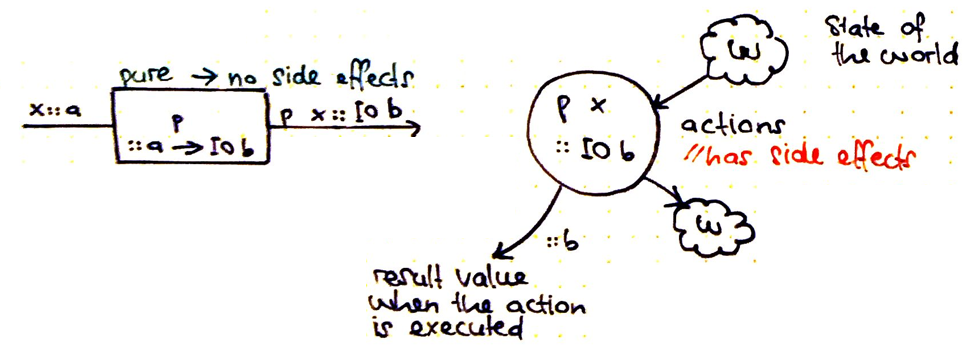
\includegraphics[width=1\textwidth]{figures/pureHaskellFunctions.png}
\caption{Pure Functions}
\end{figure}

\begin{figure}[H]
\centering
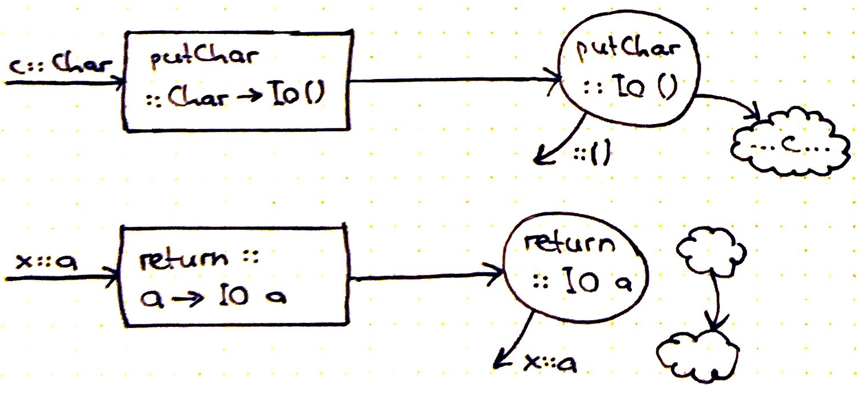
\includegraphics[width=1\textwidth]{figures/ioHaskellFunction.png}
\caption{IO Function}
\end{figure}

\begin{figure}[H]
\centering
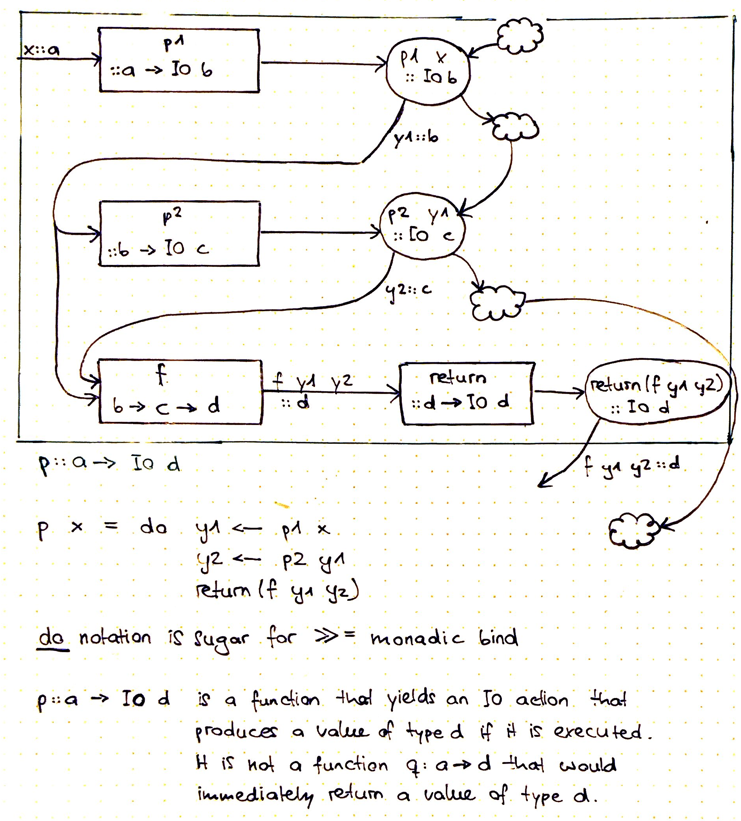
\includegraphics[width=1\textwidth]{figures/doHaskell.png}
\caption{Do Haskell}
\end{figure}

With the do notation, one is able to interact with the world multiple
times and concatonate the actions.

\textbf{p :: a -\textgreater{} IO d} is a function that yields an IO
action that produces a value of type d if the IO is executed. It is not
a function \textbf{q : a -\textgreater{} d} that would immediately
return a value of type d.

\clearpage